\begin{table}[t]
  %\resizebox{\textwidth}{!}{%
  \makebox[\textwidth][c]{
 {\scriptsize
  \begin{tabular}{@{}ll@{}}
  \toprule
  Event                 & Sample tweets \\ \midrule
  Libya Hotel Attack    & \textit{\begin{tabular}[c]{@{}l@{}}
  Gunmen possibly linked to Islamic State attack hotel popular with foreigners in Libyan capital Tripoli -officials {\tt <URL>}\\ 
  \#Libya forces surround luxury hotel in \#Tripoli where gunmen have taken hostages after car bomb attack - Reuters/AP\\ 
  %Gunmen at Libyan luxury hotel take hostages; 3 guards dead {\tt <URL>} via AP \#news
  \end{tabular}}                                                \\ \midrule
  Oscar Pistorius Trial & \textit{\begin{tabular}[c]{@{}l@{}}
  %Oscar Pistorius 'sorrow' over Reeva Steenkamp shooting - BBC News {\tt <URL>} \#news\\ 
  Oscar Pistorius pleads not guilty Monday to all 4 charges against him, marking start of Olympian's murder trial. {\tt <URL>}\\ 
  RT {\tt <mention>}: Oscar Pistorius murder trial set to begin in South Africa: {\tt <URL>}
  \end{tabular}}                                                                                                        \\ \midrule
  Nepal Earthquake      & \textit{\begin{tabular}[c]{@{}l@{}}
  Buildings down \& roads out after major 7.5 magnitude earthquake hits \#Nepal. Quake could be felt as far as Delhi {\tt <URL>}\\ 
  %Sounds bad in Kathmandu. Friends there tell me buildings down, tremors continuing. 'Really terrible'. \#nepal \#earthquake\\ 
  BREAKING: 15-year-old girl dead near Nepal border after quake brings house wall down, reports Reuters. Read more: {\tt <URL>}
  \end{tabular}} \\ \bottomrule
  
  \end{tabular}%
  }
  }
  %}
  \caption{Sample tweets for each event.}\label{tab:sample}
\end{table}

\section{Case Studies}
\label{sec:experimental}

We describe the case studies, the data, and the experiment we performed to
validate our representation.

\subsection{Datasets}

%We follow a similar approach to Kalyanam et al.~\cite{kalyanam2016prediction}.
%
%We collected tweets using the Twitter Search API using selected news accounts
%as seeds for extracting newsworthy search terms.
%
%Given a set of verified news accounts in Twitter (such as BBCNews, CNN, Al
%Jazeera, etc.), we identify the most common keywords across their tweets
%published every hour, and then we use those keywords as search terms in the
%Twitter API. \footnote{The full list of news accounts is listed in
%\url{https://github.com/mquezada/twitter-event-detection/blob/master/settings.py}}
%The data collection methodology is as follows. 
% %
% Every hour we fetch the latest tweets for each one of the seed accounts. 
% %
% Our assumption is that if an important event is happening in a certain moment
% in time, then several news accounts will be reporting on that event shortly
% after.
% %
% After the removal of stopwords, punctuation, URLs, hashtags, mentions, and
% converting words to lowercase, we tokenize each headline and find named
% entities, such as person names, locations, product names, organizations, etc.
% %
% This is possible due that the selected accounts generally employ formal
% language in their tweets. 
% %
% Then we find common subsets of tokens across the tokenized headlines, using an
% ad-hoc method resembling frequent itemset mining. 
% %
% Finally, from each common subset, we search for more related tweets in the
% Twitter Search API using the top 3 ranked terms for the next hour until the
% next batch of keywords is extracted. The source code of the data collection
% methodology is
% available\footnote{\url{https://github.com/mquezada/twitter-event-
% detection/}}.
%
For the case studies, we selected three events from our dataset (see
Chapter~\ref{chapter:data}). Namely, a terrorist attack (2015 Libya Hotel
Attack), a long-lasting event (2014 Oscar Pistorius Trial), and a natural
disaster (2015 Nepal Earthquake).
%
%Each event has different scales and levels of redundancy. 
%
We report duration in days (corresponding to the amount of days encompassing at
least 95\% of the tweets), total tweets, retweets, and unique resolved URLs
(Table~\ref{tab:datasets}).
%
We also show example tweets (Table~\ref{tab:sample}).


\begin{table}[h]
  \centering
  \begin{tabular}{@{}lrrrr@{}}
  \toprule
  Name                  & Duration & Tweets & Retweets & URLs  \\ \midrule
  Libya Hotel Attack    & 8 days   & 28,616 & 12,280 (43\%)  & 3,385            \\
  Nepal Earthquake      & 1 day   & 522,434 & 363,102 (70\%) & 22,661          \\ 
  Oscar Pistorius Trial & 70 days  & 113,189 & 26,307 (23\%)  & 9,335           \\ \bottomrule
  \end{tabular}
  \caption[Datasets for case studies.]{Datasets for case studies. The duration of each event is calculated as the amount of days that covers at least 95\% of the tweets in the dataset.}
  \label{tab:datasets}
\end{table}


\paragraph{2015 Libya Hotel Attack.} 
%
In January 27, 2015, a luxury hotel in Tripoli was attacked by men affiliated
with
ISIL.\footnote{\url{https://en.wikipedia.org/wiki/2015_Corinthia_Hotel_attack}
(Accessed: 2019-01-30)}. 
%
Attackers detonated a car bomb outside the hotel, killed security personnel and
guests, and took hostages afterwards. 
%
We filtered our data using keywords such as {\tt libya}, {\tt luxury}, {\tt
hotel}, or {\tt attack}. 
% The tweets ranged from July 2012 to January 27, 2015. The existence of
% older tweets is explained by the retrieval of retweets and older tweets
% mentioning the extracted keywords, although more than 95\% of the tweets fall
% within one week before or at the day of the attack. 
The dataset consists of 28,604 tweets (with 12,280 or 43\% of them being
retweets), 25,683 different short and 3,385 unique URLs after expanding the
short URLs. 
%
We found that 5,759 short URLs were unable to be resolved (due to be
inaccessible at the time of the resolution).

On the other hand, due to the occurrence of keywords such as {\tt luxury},
several unrelated tweets appeared in the dataset, such as the following:

\begin{itemize}
\item {\it Cheers {\tt <mention>}, named Best Luxury Hotel in The Netherlands by {\tt <mention>}!}
\item {\it New York's dazzling Baccarat Hotel opens this March, and it looks set to be a corker}
\item {\it What are your thoughts on this distinctive new hotel planned for development in China?}
\end{itemize}

% %%

\paragraph{2015 Nepal Earthquake.} 
%
In April 25, 2015, Nepal was struck by a 7.8 $\text{M}_\text{W}$ earthquake,
killing nearly 9,000
people\footnote{\url{https://en.wikipedia.org/wiki/April_2015_Nepal_earthquake}
(Accessed: 2019-01-30)}. There were historical buildings destroyed, an avalanche
in Mount Everest, and several people killed by the earthquake.
%
The dataset consists of 522,434 tweets, with the 70\% of them being retweets.
%
Also, 60,632 of the short URLs were unable to be resolved.

%%

\paragraph{2014 Trial of Oscar Pistorius.} 
%
The trial of Oscar Pistorius started on March 3, 2014, and in October, 2014 a
judge sentenced him for a maximum of 5 years for homicide; in 2015 and 2016 he
received more
sentences\footnote{\url{https://en.wikipedia.org/wiki/Trial_of_Oscar_Pistorius}
(Accessed: 2019-01-30)}.
% 
The dataset consists of 113,189 tweets, with 23\% of them being retweets.
%
Also, 21,807 short URLs were unable to be resolved.





\subsection{Experimental setting}

\paragraph{Preprocessing.}
%
To generate the representation for each event, we discarded all tweets that have
more than two URLs or more than three hashtags, as we consider them as potential
spam tweets. 
%
Note that some spam tweets may not fall into this filter.
%
We resolved every shortened URL mentioned in the tweets by following redirects. 
%
Even though the tweet meta-data may include the URLs as before they were
shortened by the Twitter platform, they are often shortened by additional
external services (e.g., {\tt bit.ly}) even more than once.
%
Also, we removed all query strings from the URLs, with some exceptions, which
for some sites they are relevant for identifying the resource (e.g., {\tt ?id=},
{\tt ?fbid=}, {\tt ?v=}, etc.).

%%

\paragraph{Model generation.} 
%
We discarded all URLs that co-occurred with 3 or more other URLs in the same
tweets. 
%
Then, we computed the representation for each event by identifying connected
components in the graph of tweets and URLs, considering only components with
URLs.
%
This resulted in 2,957 documents for the Libya event, 20,984 for the Nepal
event, and 9,092 for the Pistorius event.

%%

\paragraph{Document generation.}
%
We used fastText~\cite{bojanowski2016enriching} to produce dense vectors from
the documents.
%
We choose fastText due to its capability to encode sub-word information into the
embeddings and to encode some out-of-vocabulary words, resulting in better
quality embeddings for rare or uncommon words. 
%
This is useful in the context of social media, as there are many words with
misspellings. 
%
For the generation of document vectors, we took all the tweets in a document,
and obtained the vector of each word in each tweet.
%
Then, we took the sum of the vectors of the words in the document.
%
We trained 300-dimension word embeddings using our dataset consisting of of 193
million event-related tweets (3 billion words).
%
Note that the training of vectors can be done off-line and is done only once.


\subsection{Validation of Sub-Topic Detection Task}

To validate our representation, we produced a ground-truth using a sample of
tweets.
%
The ground-truth represented sub-topics in each event. 
%
We then computed clusters from each event in order to validate the effectiveness
of our representation.
%
The clusters were found in two settings: using the documents generated from our
representation, as described above, and from documents generated from individual
(raw) tweets.
%
Finally, the clusters in both settings were compared against the ground-truth
towards determining if our representation preserved topical information about
the events.

%%

\begin{figure}[t]
    \centering
    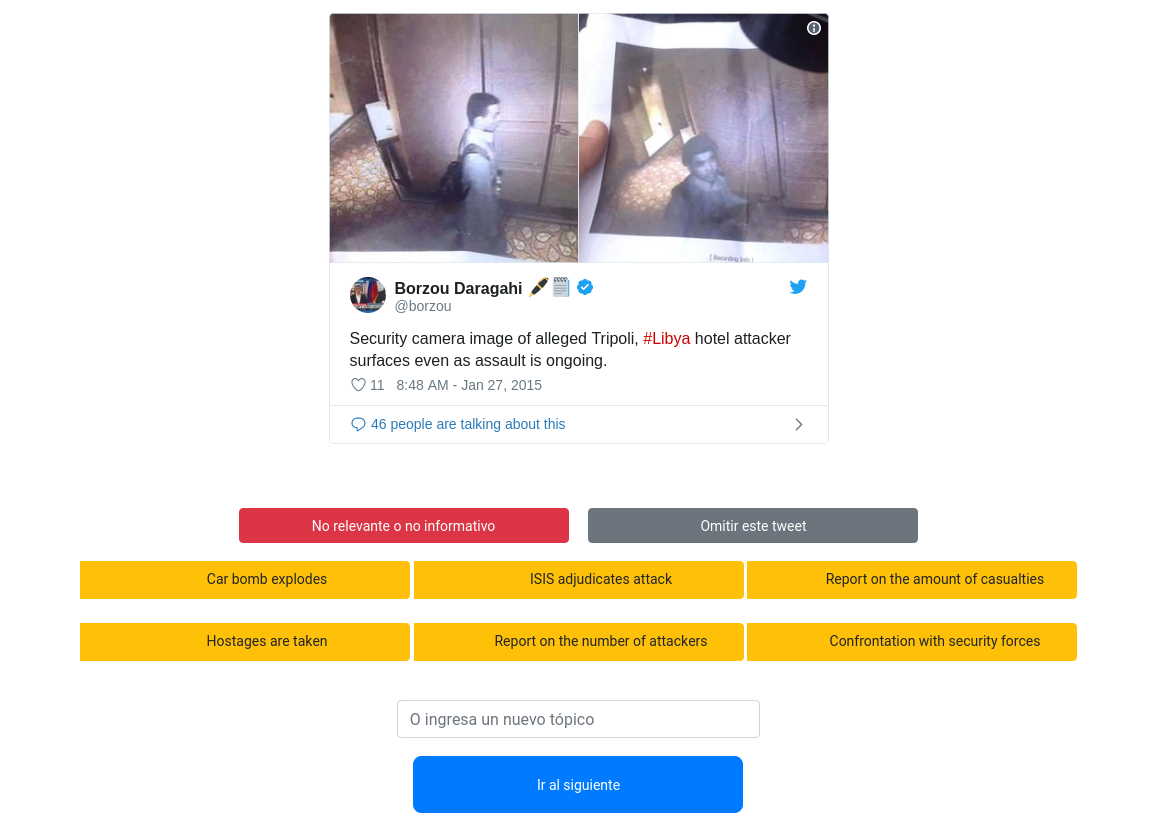
\includegraphics[width=.8\textwidth]{figures/url-model/label.png}
    \caption[Web interface for labeling tweets.]
    {Web interface for labeling tweets. In the top section a tweet is displayed.
    In the middle section, a list of options is displayed: a topic for each
    button, plus the option to mark a tweet as {\it non relevant or not
    informative}, or to skip it. In the bottom part of the interface, there is
    the possibility to add a custom topic, and then to continue with the next
    tweet. The user can select as many topics as they desire.}\label{fig:gt-web} \end{figure}%

\paragraph{Ground-truth generation.}
%
Sixteen people --mainly Computer Science undergrad and grad students-- labeled
tweets independently using a custom Web interface.
%
The interface displayed a tweet and a list of labels, and each user could assign
one or more labels to a tweet, mark the tweet as ``non relevant or not
informative'', or skip it if unsure (Figure~\ref{fig:gt-web}).
%
Some tweets may refer to more than one sub-topic, so we preferred that users
felt free to assign as many labels as they prefer.
%
The action of a user assigning labels to a tweet is referred as an evaluation,
and we imposed a limit of three evaluations per tweet.
%
This way, if three users evaluate the same tweet, that tweet will not be showed
again in the interface.

% \begin{center}
% \noindent\fbox{% 
%   \parbox{.95\textwidth}{% 
%   \it
%   The goal of this task is to assign descriptive labels to tweets.
%   %
%   With these labels we can validate a methodology to model news information
%   using tweets.

%   There are three news events available, described below. 
%   %
%   The corresponding tweets can be relevant to the event (by describing some
%   aspect of it), or not (e.g, spam, conversations).

%   %%

%   For example, if the event is an earthquake, a relevant tweet is one that 
%   informs about the magnitude, the casualties, etc.
%   %
%   A irrelevant or non informative tweet could mention the word ``earthquake'',
%   but do not describe anything about the event, or it is about something else
%   and not about the target event.
  
%   %%

  
%   Te pedimos seguir los pasos descritos abajo, y luego, al comenzar la tarea:
  
%   Escoger el o los tópicos más apropiados para cada tweet (puedes elegir más de
%   uno) Si no encuentras el tópico que crees que corresponde, puedes escribirlo
%   en el campo de texto correspondiente Si consideras que el tweet no entrega
%   información sobre el evento, o bien es totalmente irrelevante a éste, presiona
%   "No relevante o no informativo" Si no estás seguro/a de qué hacer, presiona
%   "Omitir este tweet" Si estás listo/a para continuar, presiona "Enviar" Repite
%   el proceso para el siguiente tweet Tras unos 20 o 30 minutos, vuelve a esta
%   página y pasa al siguiente evento. Estas instrucciones también están
%   disponibles en la interfaz de la tarea. Si tienes problemas con algunas
%   palabras en inglés, puedes usar algún recurso externo (como Google Translate)
%   para ayudarte. También puedes hacer click en los enlaces presentes en cada
%   tweet, pero consideramos que no es necesario. Precaución ya que algunos
%   enlaces pueden ya no estar disponibles o apuntar a sitios potencialmente
%   maliciosos.
  
%   Te pedimos al menos una hora para etiquetar tweets (unos 20 a 30 minutos por
%   cada evento).
  
%   No es necesario que destines una hora de corrido. Puedes salir y volver en
%   otro momento usando el mismo usuario y clave.
  
%   Entre más tweets etiquetes, ¡mucho mejor para nuestra evaluación! Muchas
%   Gracias :-)

%   }%
% }
% \end{center}



%
We manually generated the list of labels to be displayed in the interface by
looking into news reports in the Web.
%
The lists of labels are the following:

\begin{itemize}
  \item {\bf Libya Attack:}
  \begin{enumerate}
    \item {\it Car bomb explodes}
    \item {\it ISIS adjudicates attack}
    \item {\it Report on the amount of casualties}
    \item {\it Hostages are taken}
    \item {\it Report on the number of attackers}
    \item {\it Confrontation with security forces}
  \end{enumerate}
  \item {\bf Nepal Earthquake:}
  \begin{enumerate}
    \item {\it Avalanche in Mount Everest}
    \item {\it Death toll}
    \item {\it Reports on the magnitude of the earthquake}
    \item {\it Rescue of people}
    \item {\it Ways to help}
    \item {\it International aid}
    \item {\it Destruction of historical buildings}
    \item {\it Humanitarian crisis}
    \item {\it Destruction of buildings}
    \item {\it Replicas of the earthquake}
  \end{enumerate}
  \item {\bf Pistorius Trial:}
  \begin{enumerate}
    \item {\it Oscar Pistorius apologizes}
    \item {\it Oscar Pistorius vomits on court}
    \item {\it Oscar Pistorius removes his prosthesis}
    \item {\it Psychiatric evaluation}
    \item {\it Final arguments}
    \item {\it Pistorius pledges innocence}
    \item {\it Paddy Powers}
    \item {\it Witnesses}
    \item {\it Police under investigation}
    \item {\it Interrogatory}
    \item {\it Shooting in a restaurant}
  \end{enumerate}
\end{itemize}

To select the tweets to be displayed in the interface, we first removed all
duplicated tweets.
%
For this, we only considered the text in the tweets, but not the URLs.
%
This way, all the tweets sharing the same text would receive the same labels.
% 
Then, we distributed the resulting tweets in the interface in such a way that
there were roughly no underrepresented sub-topics.
%
For this, we manually produced a list of keywords for each label, and for each
label ranked the tweets using Okapi BM25;  in the interface, a random label was
chosen and the corresponding ranked tweet was presented.


Finally, to assign a ground-truth label to a tweet, we selected the label users
chose the most for that tweet.
%
This resulted in 401 labeled tweets (1339 labels in total) for the Libya event,
368 (531 labels) for Nepal, and 85 (362 labels) for Pistorius.

%%

\paragraph{Validation using clustering.}
%
As our goal is to compare event representations, we chose k-means as a simple
baseline to validate the effectiveness of our model.
%
To find sub-topics, we ran k-means with different numbers of clusters, using our
representation and raw tweets.
%
For the baseline, we considered each tweet as a document, that is, we computed
the sum of word vectors for each tweet individually.
%
We report normalized mutual information, purity, and entropy for each event,
using the available labels in both settings (Figures~\ref{fig:purity},
\ref{fig:nmi}, \ref{fig:entropy}).
%
Note that the measures were done only on the labeled tweets, that is, as if the
unlabeled tweets did not exist in the clustering solution.

%%

We observe that with our representation, the clustering outperforms the baseline
in most cases. 
%
In the case of the Nepal event, our representation had better purity, NMI and
entropy. 
%
In the case of Pistorius, the measures are very similar. 
%
However, in the case of Libya, our representation matches the baseline after a
certain number of clusters, except in the entropy measure
(Figure~\ref{fig:entropy}).
%
We believe this is because the Libya event has more unrelated (spam and
irrelevant) tweets, and the model captures more information about unrelated
topics, as they use more URLs.
%
And in terms of running time, we observed that k-means under the representation
runs one order of magnitude faster than the baseline (Figure~\ref{fig:times}). 
%
These results suggest that our representation is capable of preserving topical
information about the target event, with reduced time required to identify this
kind of information. 
%

\begin{figure}
  \centering
  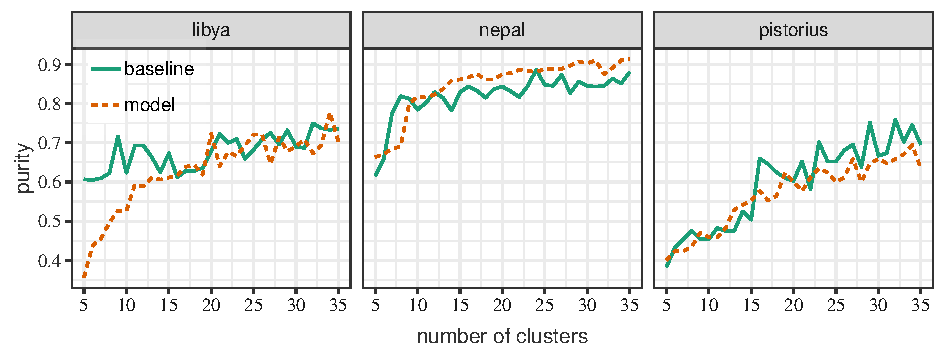
\includegraphics[width=\textwidth]{figures/url-model/purity}
  \caption{Purity for different numbers of clusters computed from each event.}\label{fig:purity}
\end{figure}%

\begin{figure}
    \centering
    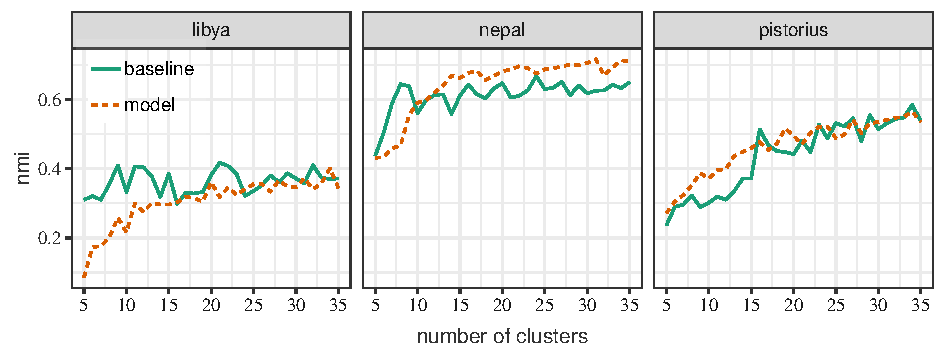
\includegraphics[width=\textwidth]{figures/url-model/nmi} 
    \caption{Normalized Mutual Information for different numbers of clusters computed from each event.}\label{fig:nmi}
\end{figure}

\begin{figure}
  \centering
  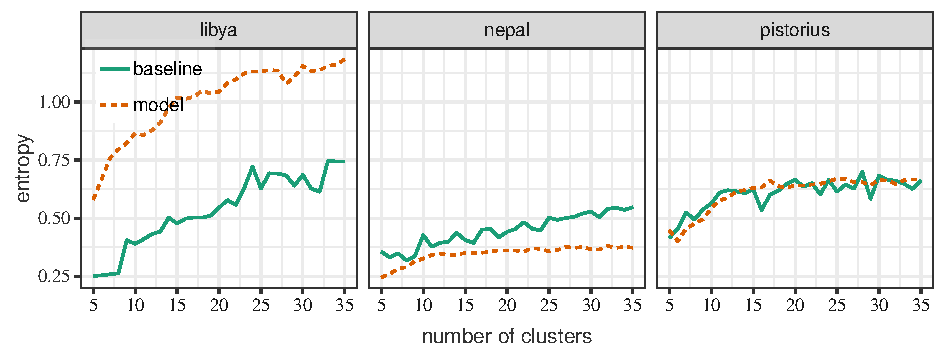
\includegraphics[width=\textwidth]{figures/url-model/entropy} 
  \caption{Entropy for different numbers of clusters computed from each event.}\label{fig:entropy}
\end{figure}


\begin{figure}
  \centering
  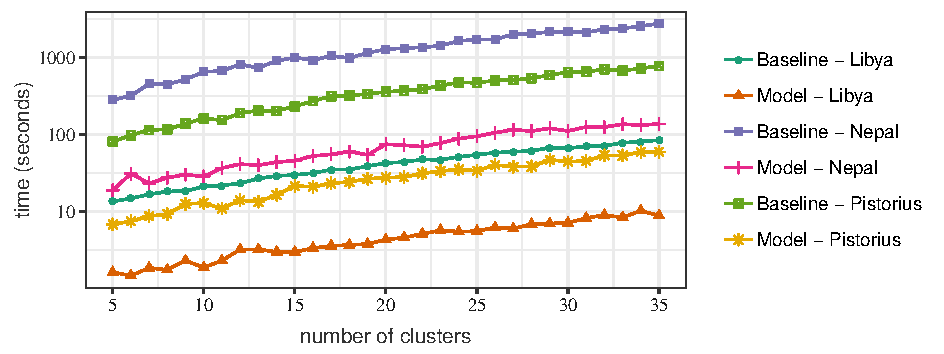
\includegraphics[width=\textwidth]{figures/url-model/times}
  \caption{Running times for clustering for each event.}\label{fig:times}
\end{figure}%